
\chapter{Design}
\section{Analysis Review}
\section{Hardware Specification}
\subsection{STM32}
microcontroler
\subsection{BMI088 IMU Sensor}
gyroscope and acelerometer
\subsection{SIM7600E-H} 
The module SIM7600E-H, developed by SIMCom, is a 4G/3G/2G LTE module that comunicates via UART commads using an intern parser described on the module datasheet. 
The waveshare Board with the module, comes with a set of extra functionalities for extra support to the module normal usage.

The following image, taken from the Waveshare board datasheet, lists the hardware features.
\begin{figure}[H]%não estou gostando dessa foto
    \centering
    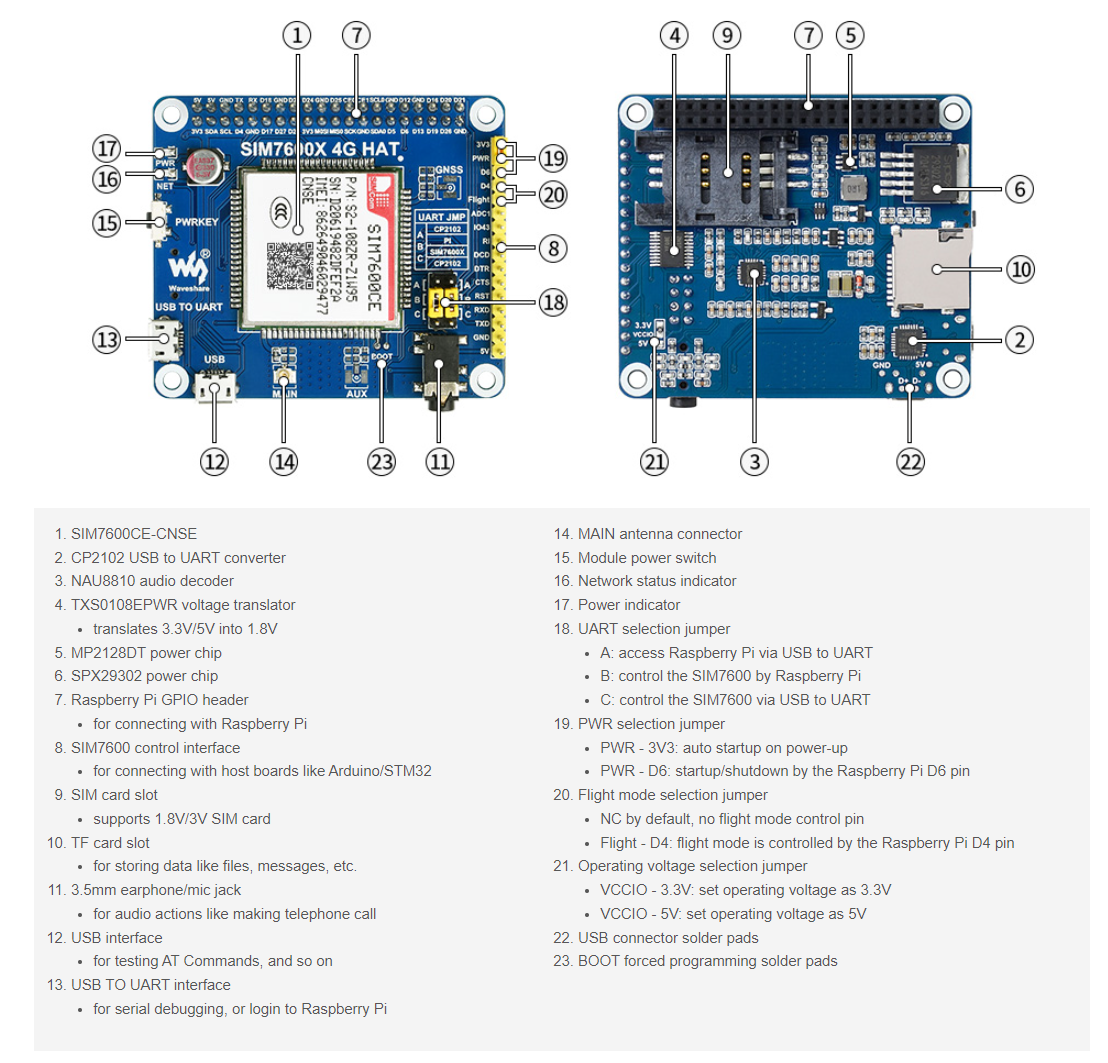
\includegraphics[width=1\textwidth]{images/chapter/design/SIM7600_board.png}
    \caption{SIM7600 datasheet}
    \label{fig:SIM7600 datasheet}
\end{figure}

The hardware configurations, as idicated on the datasheet should follow the leading steps.
%hw config

As for the UART communication, the list of commads are listed on the datasheet. 
As for better flow, here are listed the commadsused along the project and their functionalities. 
%commmand list
\section{Tools and COTS}
\subsection{Tools}
\subsection{COTS}
\subsubsection{GPS and 4G module}
\subsubsection{Inkscape}
\subsubsection{draw.io}
\subsubsection{STM32 CUBEmx}
\subsubsection{\LaTeX}
\section{Software Specification}
\section{Theorical Concepts}